\usepackage{xeCJK}
\usepackage{tikz,graphicx}    
\usepackage{booktabs}       
\usepackage[normalem]{ulem}   
\usepackage{rotating}       
\usepackage{cleveref}       
\usepackage{hyperref}       
\usepackage[absolute,overlay]{textpos}
\usepackage{xltxtra} % “Extras” for LATEX users of XETEX

\hypersetup{pdfpagemode=FullScreen}
\hypersetup{colorlinks=false}


\setbeamertemplate{navigation symbols}{} % remove navigation symbols in beamer
\setbeamertemplate{title page}[empty]    % Setting up your own title page template
\setbeamercovered{transparent}           % Transparency in itemizing

\addtobeamertemplate{title page}{
\tikz[overlay,remember picture] \node[opacity=0.3, at=(current page.center)] {
   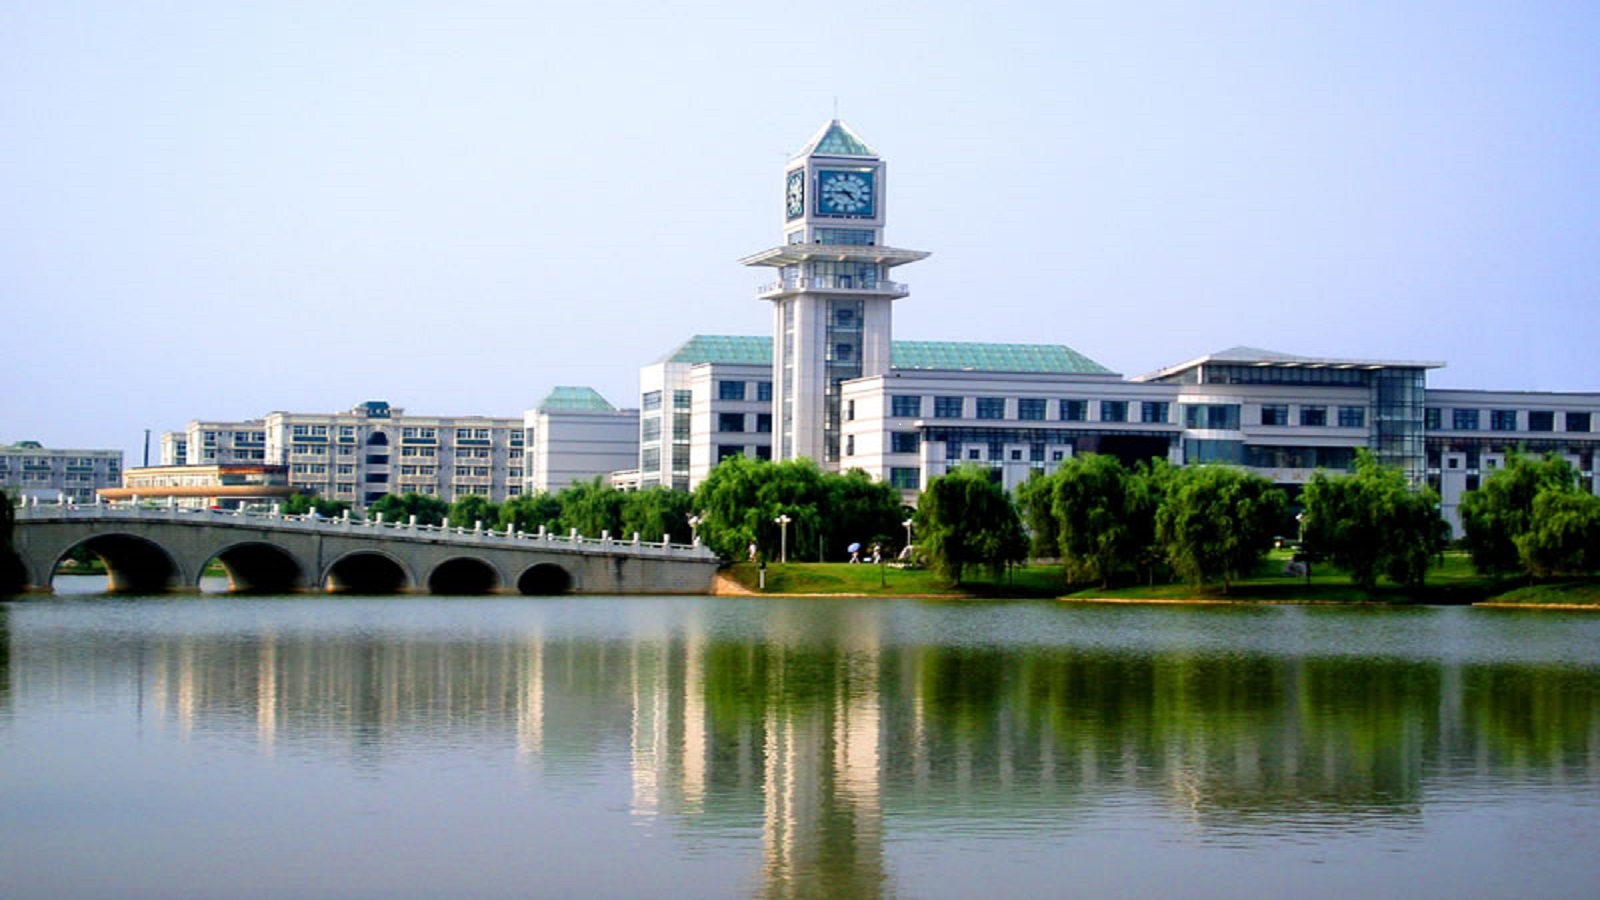
\includegraphics[width=\paperwidth,height=\paperheight,]{./figureFiles/znufebg169.jpg}};
}

%%%%%%%%%%%%%%%%%%%%%%%%%%%%%%%%%%%%%%%%%%%%%%%
% \institute{
%   {中南财经政法大学} \\
%   {\tiny 统计与数学学院} \\
%   \smallskip                                          
%   \emph {\tiny datalab026a@qq.com}                      
% }

% \institute{
%     {Zhongnan University of Economics and Law} \\
%     {\tiny School of Statistics and Mathematics} \\
%     \smallskip                                          
%     \emph {\scriptsize datalab026a@qq.com}                      
% }
%%%%%%%%%%%%%%%%%%%%%%%%%%%%%%%%%%%%%%%%%%%%%%%%%

% \usefonttheme{professionalfonts} % using non standard fonts for beamer
% \usefonttheme{serif}     % default family is serif
% \usepackage[T1]{fontenc} % Standard package for selecting font encodings
% \usepackage{lmodern}     % Latin modern fonts in outline formats

% Chinese font support

\setmainfont{Noto Serif}
\setsansfont{Noto Sans}
\setmonofont[Mapping=tex-ansi]{Noto Mono}

\setCJKmainfont{Noto Sans CJK SC}
\setCJKsansfont{Noto Sans CJK SC}
\setCJKmonofont{Noto Sans CJK SC}

\usefonttheme{default}

\setbeamerfont{title}{size=\Large,series=\bfseries,parent=structure}
\setbeamerfont{subtitle}{size=\small,series=\bfseries,parent=structure}
\setbeamerfont{section in head/foot}{size=\tiny,series=\bfseries}
\setbeamerfont{section in toc}{size=\large,series=\bfseries,parent=structure}
\setbeamerfont{frametitle}{series=\bfseries}
\setbeamerfont{author}{size=\small}
\setbeamerfont{date}{size=\scriptsize} 

\setbeamertemplate{bibliography item}[mybibitem]
\setbeamerfont{bibliography entry author}{shape=\upshape,series=\bfseries,size=\normalsize}%
\setbeamerfont{bibliography entry title}{shape=\upshape,size=\small,series=\mdseries}
\setbeamerfont{bibliography entry journal}{shape=\upshape,size=\small,series=\mdseries}
\setbeamerfont{bibliography entry note}{shape=\upshape,size=\small,series=\mdseries}

\setbeamerfont{itemize/enumerate body}{size=\small}
\setbeamerfont{itemize/enumerate subbody}{size=\footnotesize}
\setbeamerfont{itemize/enumerate subsubbody}{size=\scriptsize}

\setbeamerfont{block title}{size=\normalsize,series=\bfseries,parent={structure,block body}}



\definecolor{texpurple}{HTML}{522D80}
\definecolor{texorange}{HTML}{F66733}
\definecolor{texblue}{HTML}{2B3856}
\definecolor{antiquewhite}{rgb}{0.98, 0.92, 0.84}
\definecolor{aliceblue}{rgb}{0.94, 0.97, 1.0}
\definecolor{lighttaupe}{rgb}{0.7, 0.55, 0.43}
\definecolor{mediumtaupe}{rgb}{0.4, 0.3, 0.28}
\definecolor{taupe}{rgb}{0.28, 0.24, 0.2}
\definecolor{darktaupe}{rgb}{0.28, 0.24, 0.2}
\definecolor{camouflagegreen}{rgb}{0.47, 0.53, 0.42}

% \setbeamercolor{frametitle}{fg=texpurple,bg=white}
% \setbeamercolor{title}{fg=texpurple,bg=white}
% \setbeamercolor{local structure}{fg=texpurple}
% \setbeamercolor{section in toc}{fg=texpurple,bg=white}
% \setbeamercolor{section in toc shaded}{fg = texpurple}
% \setbeamercolor{subsection in toc}{fg=texblue,bg=white}
% \setbeamercolor{item projected}{fg=texpurple,bg=white}
% \setbeamercolor{caption}{fg = texpurple}
% \setbeamercolor{caption name}{fg = texpurple}
% \setbeamercolor{normal text}{fg = black}
% \setbeamertemplate{itemize item}{\color{texpurple}$\bullet$}
% \setbeamertemplate{itemize subitem}{\color{texpurple}\scriptsize{$\bullet$}}

\definecolor{bottomcolour}{rgb}{0.32,0.3,0.38}
\definecolor{middlecolour}{rgb}{0.08,0.08,0.16}

\setbeamerfont{title}{size=\Huge}
\setbeamercolor{structure}{fg=white}
\setbeamertemplate{frametitle}[default][center]

\setbeamercolor{normal text}{bg=black, fg=white}
\setbeamertemplate{background canvas}[vertical shading]
[bottom=bottomcolour, middle=middlecolour, top=black]

\setbeamertemplate{itemize item}{\lower3pt\hbox{\Large\textbullet}}
\setbeamerfont{frametitle}{size=\huge} 
% problock
\newenvironment<>{problock}[1]{%
  \begin{actionenv}#2%
      \def\insertblocktitle{#1}%
      \par%
      \mode<presentation>{%
       \setbeamercolor{block title}{fg=texorange!80!white,bg=middlecolour!20!darktaupe}
       \setbeamercolor{block body}{fg=texblue!50!white,bg=middlecolour!50!darktaupe}
       \setbeamercolor{itemize item}{fg=darktaupe}
       \setbeamercolor{enumerate item}{fg=darktaupe}
       \setbeamertemplate{itemize item}[triangle]
     }%
      \usebeamertemplate{block begin}}
    {\par\usebeamertemplate{block end}\end{actionenv}}
\useoutertheme[right,height=0pt,width=0.12\paperwidth]{sidebar}
\setbeamertemplate{sidebar canvas right}[vertical shading][bottom=bottomcolour, middle=middlecolour, top=black] 
% \setbeamertemplate{sidebar canvas right}[horizontal shading][left=bottomcolour!20!white,right=white] 

\setbeamercolor{title in sidebar}{fg=taupe}  
\setbeamercolor{author in sidebar}{fg=taupe}
\setbeamercolor{section in sidebar}{fg=lighttaupe}
\setbeamercolor{section in sidebar shaded}{fg=darktaupe}
\setbeamercolor{subsection in sidebar}{fg=lighttaupe}
\setbeamercolor{subsection in sidebar shaded}{fg=darktaupe}

\setbeamerfont{title in sidebar}{family=\sffamily} 
\setbeamerfont{author in sidebar}{family=\sffamily} 
\setbeamerfont{section in sidebar}{family=\sffamily} 
\setbeamerfont{subsection in sidebar}{family=\sffamily} 

\setbeamerfont{title in sidebar}{size=\fontsize{4.5}{4.5}\selectfont}
\setbeamerfont{author in sidebar}{size=\fontsize{3}{3}\selectfont}
\setbeamerfont{section in sidebar}{size=\fontsize{5}{5}\selectfont}
\setbeamerfont{subsection in sidebar}{size=\fontsize{3.5}{3.5}\selectfont}

\usetheme[hideothersubsections]{}

\makeatletter
\setbeamertemplate{section in sidebar}%{sidebar theme}
{%
  \vbox{%
    \vskip1ex%
    \beamer@sidebarformat{3pt}{section in sidebar}{\insertsectionheadnumber
~\insertsectionhead}%
  }%
}
\setbeamertemplate{section in sidebar shaded}%{sidebar theme}
{%
  \vbox{%
    \vskip1ex%
    \beamer@sidebarformat{3pt}{section in sidebar shaded}{\insertsectionheadnumber
~\insertsectionhead}%
  }%
}
\makeatother

% mathcircled
\makeatletter
\newcommand\mathcircled[1]{%
  \mathpalette\@mathcircled{#1}%
}
\newcommand\@mathcircled[2]{%
  \tikz[baseline=(math.base)] \node[draw,circle,inner sep=1pt] (math) {$\m@th#1#2$};%
}
\makeatother
\makeatletter
\define@key{Gin}{grlarge}[true]{%
    \edef\@tempa{{Gin}{width=4.25in,height=6.5in}}%
    \expandafter\setkeys\@tempa
}
\define@key{Gin}{grsmall}[true]{%
    \edef\@tempa{{Gin}{width=3.2in,height=3.8in}}%
    \expandafter\setkeys\@tempa
}
\makeatother
\setbeamertemplate{footline}{% footline add page number
\hfill\usebeamertemplate***{navigation symbols}
\hspace{1cm}\insertframenumber{}/\inserttotalframenumber}

\setbeamercolor{footline}{fg=texpurple}
\setbeamerfont{footline}{series=\bfseries}

\setbeamertemplate{caption}{%
\begin{beamercolorbox}[wd=\paperwidth, dp=0.5ex, sep=0.2ex, center]{block body}\insertcaption%
\end{beamercolorbox}%
}

\newcommand\FootText[1]{
  \begin{textblock*}{\textwidth}(0pt,\textheight)\raggedright #1 \hspace{20pt}\end{textblock*}}

\AtBeginPart{}

\AtBeginSection[]{
  \begin{frame}[c]
    \begin{center}
      \setbeamerfont{section in toc}{family=\sffamily,size=\LARGE} 
      \tableofcontents[sectionstyle=show/hide,subsectionstyle=hide/show/hide]
    \end{center}
  \end{frame}
}
\AtBeginSubsection{}
\AtBeginSubsubsection{}
\setlength{\emergencystretch}{0em}
\setlength{\parskip}{0pt}